\chapter{Grundlagen}
In diesem Kapitel werden die wichtigen Grundlagen f�r diese
Aufgabenstellung erl�utert.

\section{Verwendete Hard- und Software}

\subsection{Hardware}

Alle hier hier vorgestellten Algorithmen laufen auf einem Raspberry Pi 3 Modell B mit einer Quad Core 1.2GHz Broadcom BCM2837 64bit CPU und 1GB RAM \cite{RASPBERRY}.

\begin{figure}[hb]
	\centering
	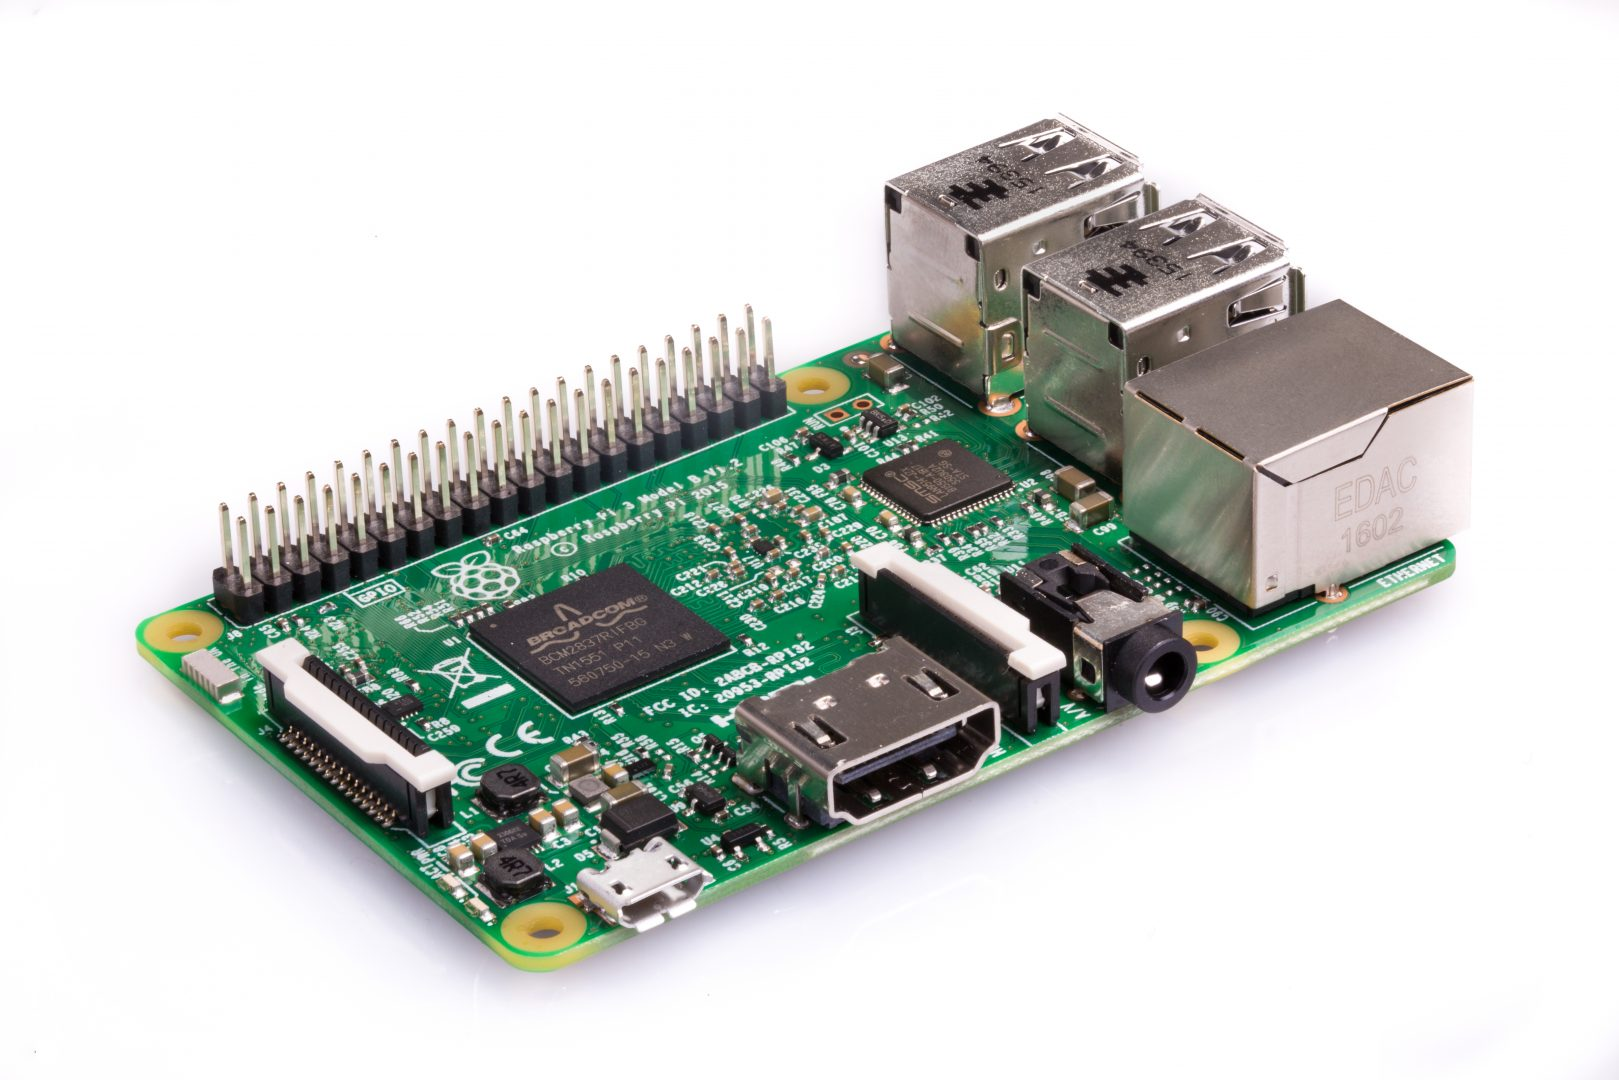
\includegraphics[scale=0.2]{bilder/Raspberry.jpg}
	\caption{Raspeberry Pi 3 Modell B,  Quelle:\cite{RASPBERRYPIC}}
	\label{fig:Raspberry}
\end{figure}

Weiter wird eine Kamera  von  Raspberry Pi Camera Module v1 mit einer Aufl�sung von 640 x 480p bei 60 fps verwendet \cite{RASPBERRYCAM}.



\subsection{Software}
Zur Programmierung der Software wird MATLAB\textregistered\ (2017b) mit Simulink\textregistered\ und dessen Emebedded Coder\texttrademark\ ,\ sowie die Image Processing Toolbox\texttrademark\ verwendet.


\begin{figure}[hb]
	\centering
	
\includegraphics[scale=0.5]{bilder/MATLABLogo.png}
	\caption{MATLAB Logo}
	\label{fig:MATLAB}
\end{figure}



